\begin{figure}[tb]
\centering
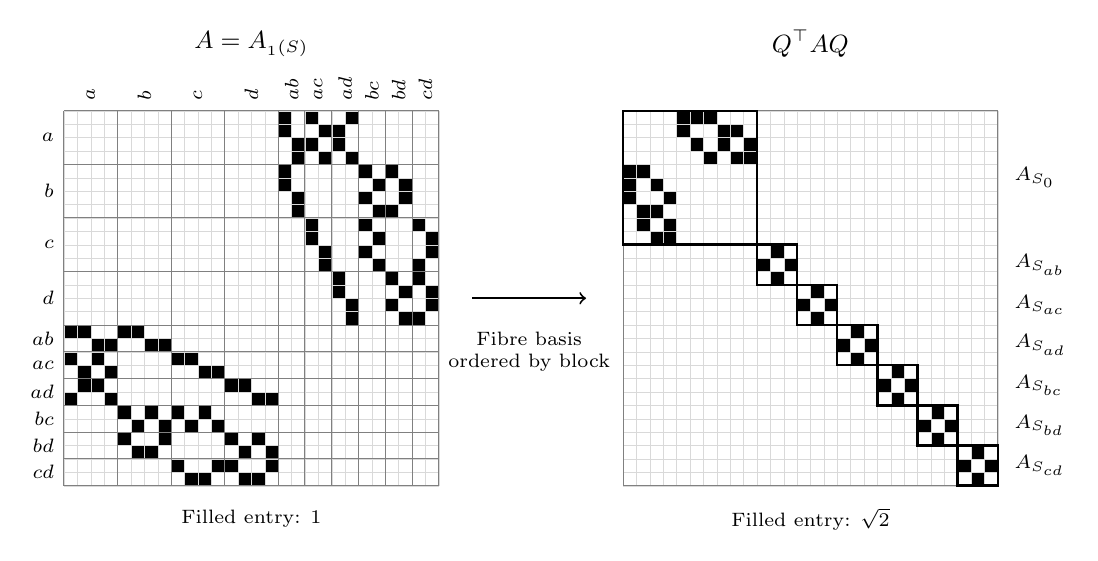
\begin{tikzpicture}[
  x=.17cm,y=-.17cm,
  entry/.style={fill=black},
  gridline/.style={draw=black!15,line width=.1pt},
  fibreline/.style={draw=black!50,line width=.35pt},
  block/.style={draw=black,line width=.9pt},
  every node/.style={font=\scriptsize,inner sep=1pt},
]
\node[font=\small] at (14,-5) {$A=A_{\CFI_1(S)}$};
\foreach \v/\e/\k in {
  0/0/0,0/1/1,0/2/2,
  1/0/0,1/3/1,1/4/2,
  2/1/0,2/3/1,2/5/2,
  3/2/0,3/4/1,3/5/2
} {
  \ifnum\v=0
    \def\fibrebits{0/0/0/1,1/0/1/0,2/1/0/0,3/1/1/1}
  \else
    \def\fibrebits{0/0/0/0,1/0/1/1,2/1/0/1,3/1/1/0}
  \fi
  \foreach \r/\first/\second/\third in \fibrebits {
    \ifcase\k\edef\bit{\first}\or\edef\bit{\second}\or\edef\bit{\third}\fi
    \pgfmathtruncatemacro{\row}{4*\v+\r}
    \pgfmathtruncatemacro{\col}{16+2*\e+\bit}
    \fill[entry] (\col,\row) rectangle ++(1,1);
    \fill[entry] (\row,\col) rectangle ++(1,1);
  }
}
\foreach \position in {0,...,28} {
  \draw[gridline] (\position,0)--(\position,28);
  \draw[gridline] (0,\position)--(28,\position);
}
\foreach \boundary in {0,4,8,12,16,18,20,22,24,26,28} {
  \draw[fibreline] (\boundary,0)--(\boundary,28);
  \draw[fibreline] (0,\boundary)--(28,\boundary);
}
\foreach \position/\name in {
  2/a,6/b,10/c,14/d,17/ab,19/ac,21/ad,23/bc,25/bd,27/cd
} {
  \node[anchor=west,rotate=90] at (\position,-.5) {$\name$};
  \node[anchor=east] at (-.5,\position) {$\name$};
}
\node at (14,30.5) {Filled entry: $1$};

\draw[->,line width=.7pt] (30.5,14)--(39,14);
\node[align=center] at (34.75,18) {Fibre basis\\ordered by block};

\begin{scope}[xshift=7.1cm]
  \node[font=\small] at (14,-5) {$Q^{\top}AQ$};
  \foreach \e/\u/\v in {0/0/1,1/0/2,2/0/3,3/1/2,4/1/3,5/2/3} {
    \pgfmathtruncatemacro{\subdivision}{4+\e}
    \foreach \endpoint in {\u,\v} {
      \fill[entry] (\subdivision,\endpoint) rectangle ++(1,1);
      \fill[entry] (\endpoint,\subdivision) rectangle ++(1,1);
    }
    \pgfmathtruncatemacro{\start}{10+3*\e}
    \foreach \r/\c in {0/1,1/0,1/2,2/1} {
      \fill[entry] ({\start+\c},{\start+\r}) rectangle ++(1,1);
    }
  }
  \foreach \position in {0,...,28} {
    \draw[gridline] (\position,0)--(\position,28);
    \draw[gridline] (0,\position)--(28,\position);
  }
  \draw[fibreline] (0,0) rectangle (28,28);
  \draw[block] (0,0) rectangle (10,10);
  \node[anchor=west] at (29,5) {$A_{S_0}$};
  \foreach \j/\e in {0/ab,1/ac,2/ad,3/bc,4/bd,5/cd} {
    \pgfmathtruncatemacro{\start}{10+3*\j}
    \draw[block] (\start,\start) rectangle ++(3,3);
    \node[anchor=west] at (29,{\start+1.5}) {$A_{S_{\e}}$};
  }
  \node at (14,30.5) {Filled entry: $\sqrt2$};
\end{scope}
\end{tikzpicture}
\caption{Block decomposition for the subdivision $S$ of $\Gamma=K_4$
on vertices $a,b,c,d$, with tree attachments omitted.
The left matrix groups the $28$ CFI vertices by fibre and uses odd parity
at $a$. Within fibres, the bit vectors are in lexicographic order,
with incident-edge coordinates ordered by their labels.
The columns of $Q$ are the fibre basis vectors from the proof, ordered
first by the ten constant directions and then by the three sign directions
over $v,e,w$ for each edge $e=vw$ of $K_4$.
The right matrix has one $10\times10$ block $A_{S_0}=\sqrt2 A_S$ and
six $3\times3$ blocks $A_{S_e}$; unfilled entries are zero.
Both CFI parities give the same right matrix.}
\label{fig:ss-cfi-blocks}
\end{figure}
